\documentclass[sigchi]{acmart}

\def\tightlist{}
\settopmatter{printacmref=false}
\renewcommand\footnotetextcopyrightpermission[1]{}

\usepackage{booktabs} % For formal tables

% Copyright
\setcopyright{none}
%\setcopyright{acmcopyright}
%\setcopyright{acmlicensed}
%\setcopyright{rightsretained}
%\setcopyright{usgov}
%\setcopyright{usgovmixed}
%\setcopyright{cagov}
%\setcopyright{licensedcagov}
%\setcopyright{cagovmixed}
%\setcopyright{licensedothergov}

% DOI
\acmDOI{10.475/123_4}

% ISBN
\acmISBN{123-4567-24-567/08/06}

%Conference
\acmConference[Business Intelligence]{Assignment 3}{January 2021}{Linz/Vienna, Austria}
\acmYear{2021}
\copyrightyear{2021}

\acmPrice{15.00}


\begin{document}
\title{Predicting the resale value of used cars}
\subtitle{Created using R Markdown}

\author{Simone Andreetto}
\affiliation{%
  \institution{01635069}
}

\author{Felix Winterleitner}
\affiliation{%
  \institution{01612776}
}

% The default list of authors is too long for headers.
\renewcommand{\shortauthors}{S. Andreetto et al.}


\begin{abstract}
This is Assignment 3 in Business Intelligence @ TU Wien in the winter term of 2020.
\end{abstract}


\keywords{Business Intelligence, R, Rmd, Spark}

\begin{teaserfigure}
  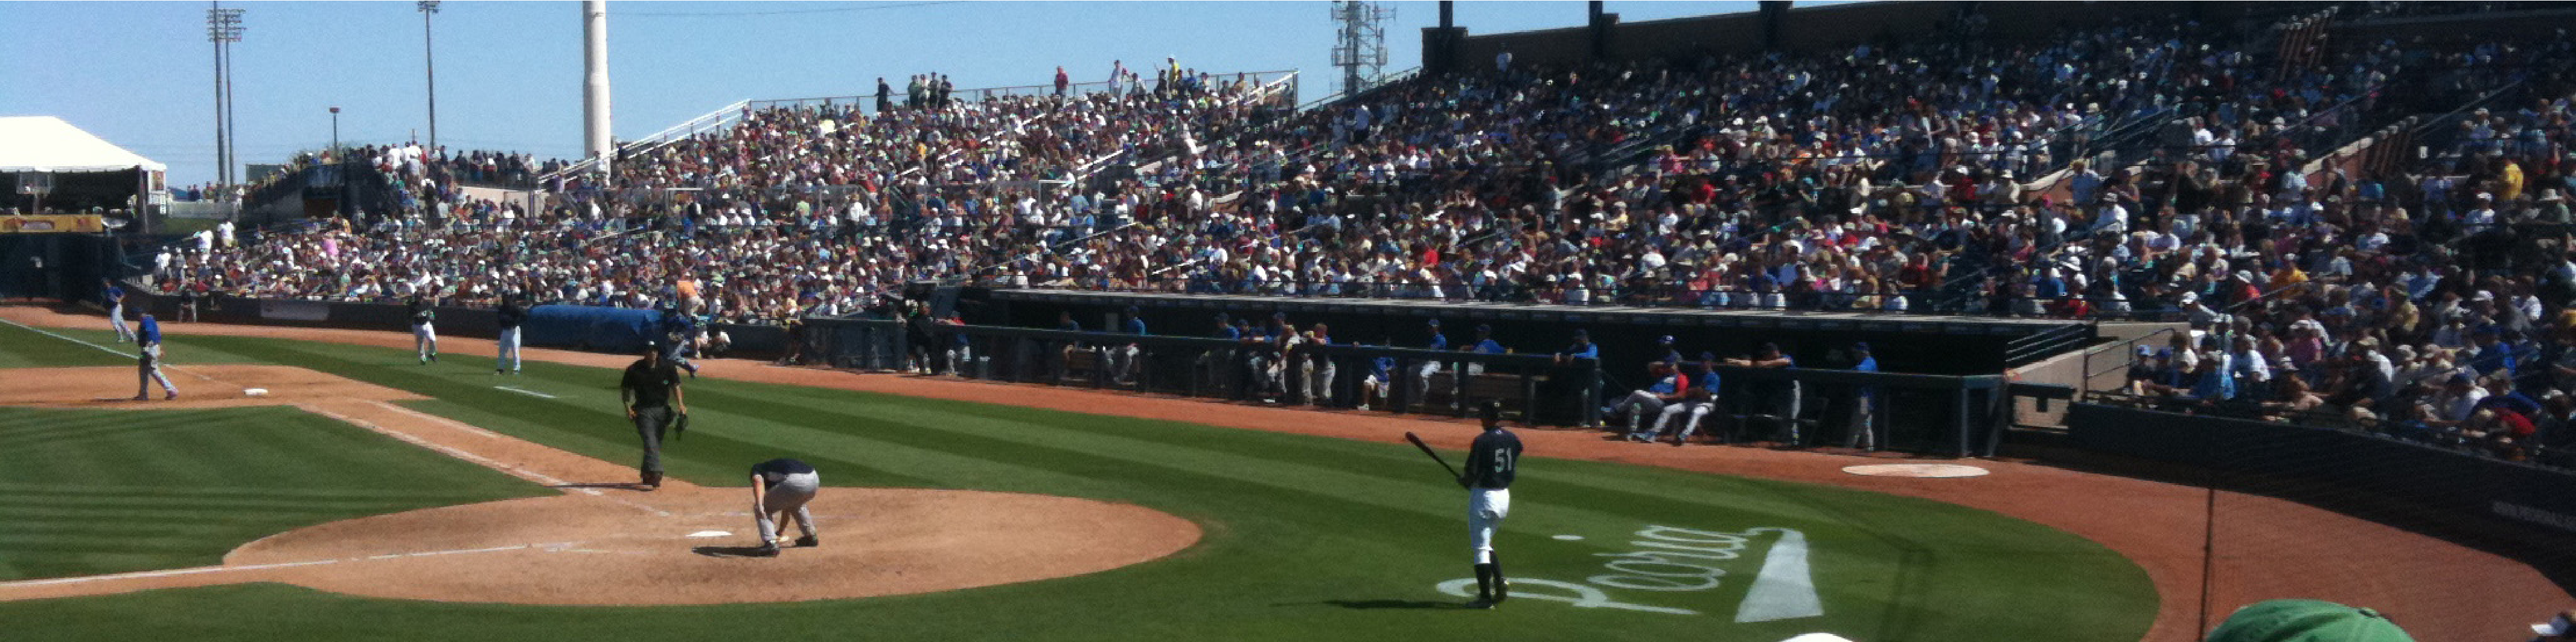
\includegraphics[width=\textwidth]{sampleteaser}
  \caption{This is a teaser}
  \label{fig:teaser}
\end{teaserfigure}


\maketitle

\hypertarget{introduction}{%
\section{Introduction}\label{introduction}}

For this project, we used a dataset found on Kaggle.com provided by user Aditya \citep{Aditya}. It contains a collection of different used car listings obtained by searching through online marketplaces using a web scraper. The dataset is split into different files, one per car brand. The brands for which data is available are:

\begin{itemize}
\tightlist
\item
  Audi
\item
  BMW
\item
  Ford
\item
  Hyundai
\item
  Mercedes
\item
  Skoda
\item
  Toyota
\item
  Vauxhall (= Opel in Great Britain)
\item
  VW
\end{itemize}

Additionally, the data set contains files with premade subsets of above mentioned car brands, for example \emph{coclass.csv}, which contains only listings for the Mercedes model C Class. We chose to only utilize the unfiltered datasets.

\hypertarget{business-understanding}{%
\section{Business Understanding}\label{business-understanding}}

\hypertarget{scenario}{%
\subsection{Scenario}\label{scenario}}

The

\begin{enumerate}
\def\labelenumi{\alph{enumi}.}
\tightlist
\item
  Define and describe a scenario in which a business analytics task based on the data set you identified should be solved
\item
  Define and describe the Business Objectives
\item
  Define and describe the Business Success Criteria
\item
  Define and describe the Data Mining Goals
\item
  Define and describe the Data Mining Success Criteria
\end{enumerate}

Citation example.\citep{Aditya}
Plot example.\textbf{The maturation of the song over time is shown in Figure \ref{fig:tribute-plot}.}

\begin{figure}
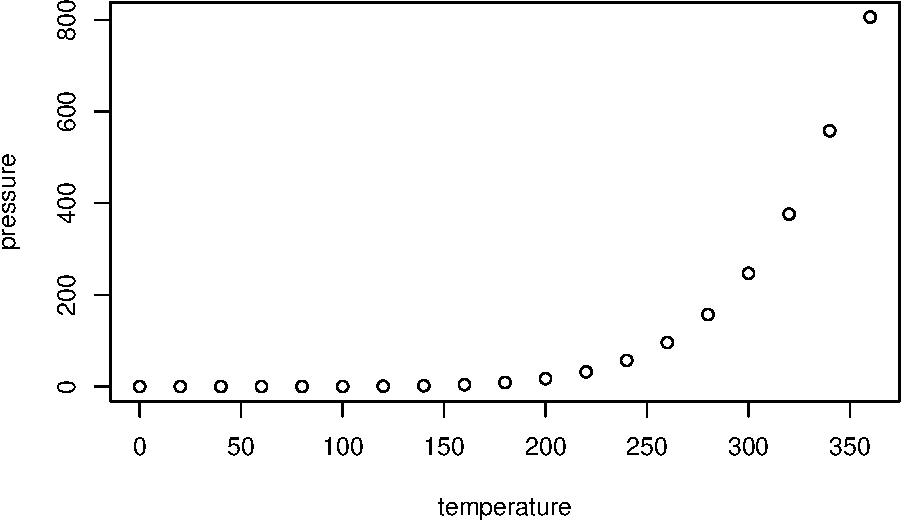
\includegraphics[width=0.98\columnwidth]{step6_files/figure-latex/tribute-plot-1} \caption{This is how great Tribute gets over time}\label{fig:tribute-plot}
\end{figure}

Small plot example.

\begin{figure*}
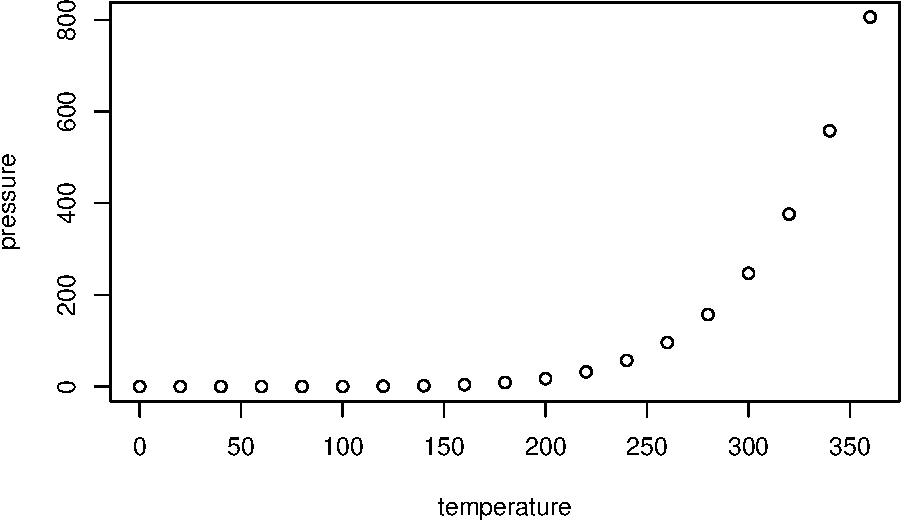
\includegraphics[width=0.98\textwidth]{step6_files/figure-latex/two-col-tribute-plot-1} \caption{This is a two-column plot of how great Tribute gets over time}\label{fig:two-col-tribute-plot}
\end{figure*}

\hypertarget{data-understanding}{%
\subsection{Data Understanding}\label{data-understanding}}

Insert content here.

Data Description Report presenting
a. Data types,
b. Statistical properties
c.~Data Quality aspects
d.~Visual Exploration of data properties and hypotheses

Table example.

\begin{table}

\caption{\label{tab:table-iris}The favorite iris' of Tenacious D.}
\centering
\begin{tabular}[t]{rrrr}
\toprule
Sepal.Length & Sepal.Width & Petal.Length & Petal.Width\\
\midrule
5.1 & 3.5 & 1.4 & 0.2\\
4.9 & 3.0 & 1.4 & 0.2\\
4.7 & 3.2 & 1.3 & 0.2\\
4.6 & 3.1 & 1.5 & 0.2\\
5.0 & 3.6 & 1.4 & 0.2\\
\addlinespace
5.4 & 3.9 & 1.7 & 0.4\\
4.6 & 3.4 & 1.4 & 0.3\\
5.0 & 3.4 & 1.5 & 0.2\\
4.4 & 2.9 & 1.4 & 0.2\\
4.9 & 3.1 & 1.5 & 0.1\\
\bottomrule
\end{tabular}
\end{table}

\hypertarget{data-preparation-report}{%
\subsection{Data Preparation report}\label{data-preparation-report}}

Insert content here.

\begin{enumerate}
\def\labelenumi{\alph{enumi}.}
\tightlist
\item
  Analyze options and potential for derived attributes (note: if the potential is considered low, these obviously do not necessarily have to be applied for your analysis, but options should be documented)
\item
  Analyze options for additional external data sources, attributes that might be useful to better address the business objectives or data mining goals (Note: this description may be hypothetical, i.e.~you are not necessarily required to actually obtain and integrate the external data for the analysis)
\item
  Describe other pre-processing steps considered, specifying which ones were applied or not applied due to which reason. (e.g.~data cleansing, transformations, binning, scaling, outlier removal, attribute removal, transcoding, \ldots) at a level of detail that ensures reproducibility of changes to the data. (Code may be supplied as supplement to the submission in case you produce your own code)
\end{enumerate}

\hypertarget{modeling}{%
\subsection{Modeling}\label{modeling}}

Insert content here.

\begin{enumerate}
\def\labelenumi{\alph{enumi}.}
\tightlist
\item
  Identify suitable data mining algorithms and select one of these as the most suitable for your experiments, providing a brief justification.
\item
  Identify the hyper-parameters available for tuning in your chosen algorithm and select one that you deem most relevant for tuning, providing a brief justification.
\item
  Define and document a train / validation / test set split, considering where necessary appropriate stratification, any dependencies between data instances (e.g.~time series data) and relative sizes of the respective subsets.
\item
  Train the model on the training set and comparing the performance on the validation set to identify the best hyper-parameter setting, explicitly documenting all parameter settings (avoid stating simply to have used ``default parameters'', focus on reproducibility of the results you report).
  188.429 Business Intelligence (VU 4,0) -- WS 2020/21 Assignment 2: Data Analytics
\item
  Report suitable performance metrics supported, where possible, by figures/graphs showing the tuning process of the hyper parameter.
\end{enumerate}

\hypertarget{evaluation}{%
\subsection{Evaluation}\label{evaluation}}

Insert content here.

\begin{enumerate}
\def\labelenumi{\alph{enumi}.}
\tightlist
\item
  Apply the final model on the test data and document performance.
\item
  Re-train the model with identical hyper-parameters using the full train and validation data and again apply it on the test data, documenting the performance
\item
  Identify and document

  \begin{enumerate}
  \def\labelenumii{\roman{enumii}.}
  \tightlist
  \item
    state-of-the-art performance from the literature using the same (albeit potentially slightly differently pre-processed) data set from the literature.
  \item
    the expected base-line performance of a trivial acceptor / rejecter or random classifier
  \end{enumerate}
\item
  Compare the performance achieved with the benchmark and baseline performances (c.f. Section 1e -- Data Mining success Criteria) according to different metrics (i.e.~overall, but also on per-class level (confusion matrix), micro/macro precision/recall in the case of classification tasks, regression errors in certain parts of the data space, \ldots{} (Note your goal is not necessarily to obtain a better result than what has been reported in the state of the art, this is not a grading criterion! On the other hand, if the performance of your classifiers is massively below the stat of the art (or even below a random baseline or trivial acceptor / rejecter) you may want to investigate the reason\ldots)
\item
  Compare the performance obtained with the Data Mining success criteria defined in the business understanding phase.
\end{enumerate}

\hypertarget{deployment}{%
\subsection{Deployment}\label{deployment}}

Insert content here.

\begin{enumerate}
\def\labelenumi{\alph{enumi}.}
\tightlist
\item
  Compare the performance obtained with respect to the needs for addressing the business success criteria and provide recommendations for deployment (fully automatic, hybrid solutions, deploying only for a part of the data space, \ldots) as well as recommendations for subsequent analysis.
\item
  Consider and briefly document potential ethical aspects as well as impact assessment / risks identified in deployment
\item
  Document aspects to be monitored during deployment, specifying triggers that should lead to intervention.
\item
  Briefly re-visit reproducibility aspects reflecting on aspects well documented and those that might pose a risk in terms of reproducibility based solely on the information provided in this report
\end{enumerate}

\hypertarget{summary-of-findings}{%
\subsection{Summary of findings}\label{summary-of-findings}}

Insert content here.

\begin{enumerate}
\def\labelenumi{\alph{enumi}.}
\tightlist
\item
  Briefly summarize your overall findings and lessons learned
\item
  (optional) Provide feedback on this exercise in general: which parts were useful / less useful; which other kind of experiment would have been interesting, \ldots{} (this section is, obviously, optional and will not be considered for grading. You may also decide to provide that kind of feedback anonymously via the feedback mechanism in TISS -- in any case we would appreciate learning about it to adjust the exercises for next year following a major re-structuring this year based on feedback obtained.)
\end{enumerate}

\bibliographystyle{ACM-Reference-Format}
\bibliography{my-bibliography}

\end{document}
